\documentclass[12pt,letterpaper]{article}

\usepackage[spanish,es-tabla,es-nodecimaldot]{babel}
\usepackage{amsmath}
\usepackage[utf8]{inputenc}
\usepackage[T1]{fontenc}
\usepackage{lmodern}
\usepackage{graphicx}
\usepackage{listings}
\usepackage{anysize} 
\usepackage{fancyhdr}
\usepackage{amsmath}
\usepackage{pdfpages}
\usepackage{graphics}
\usepackage{capt-of}
\usepackage{tabularx}
\usepackage{rotating}
\usepackage{tikz}
\usepackage[colorlinks=true,plainpages=true,citecolor=blue,linkcolor=blue]{hyperref}

\marginsize{2cm}{2cm}{2cm}{2cm}
\pagestyle{fancy}
\fancyhf{Redes de Telecomunicaciones}
\fancyhead[L]{\footnotesize UPIITA-IPN} 
\fancyhead[R]{\footnotesize 4TV2} 
\fancyfoot[R]{\footnotesize Memoría técnica}
\fancyfoot[C]{\thepage}
\fancyfoot[L]{\footnotesize La Costeña} 

\renewcommand{\footrulewidth}{0.4pt}
\renewcommand{\spanishtablename}{Tabla}
\renewcommand{\labelitemii}{$\star$}
\graphicspath{ {C:/Users/Anselmo-PC/Documents/GitHub/upiita-RedesTelecomunicaciones/MemTec/imagenes} }

\begin{document}

\includepdf[pages={1}]{portada2}

\newpage
\tableofcontents
\listoffigures
\listoftables

\newpage
\section{Antecedentes}
\subsection{La Costeña}
Conservas La Costeña, usualmente llamada La Costeña, es una marca mexicana dedicada al mercado de conservas. 
Fue fundada en 1923 por Vicente López Recines. La empresa se ha convertido en una marca importante dentro y fuera de México. 
Hoy en día, La Costeña vende sus productos en todo México y en 40 países de todo el mundo. A pesar de que sus productos al principio eran chiles, 
la empresa comenzó a producir nuevos productos como frijoles, ketchup, vegetales y otros. Las plantas de producción también han sido modificadas, 
además de que las fábricas han ganado algunos reconocimientos por los cambios en tecnología y procesos. \cite{lacostena}

\begin{figure}[ht]
    \centering
    
\includegraphics[width=0.5\textwidth]{imagenes/lacostena.jpg}
    \caption{Logotipo empresa.}
\end{figure}

\subsubsection{Misión}
Proporcionar a las familias alimentos envasados de alta calidad que preserven el buen sabor de la cocina mexicana, 
faciliten su preparación y mantenga un precio bajo, con la finalidad de que sean accesibles para todos los consumidores.

\subsubsection{Visión}
Ser la empresa líder en el mercado nacional de conservas alimenticias y con creciente presencia internacional que a 
través de los productos y servicios proporcione la mayor satisfacción a sus clientes, basándose en el desarrollo de personal 
altamente calificado y comprometido, así como el empleo de tecnología de punta para la creación de nuestros productos.

\subsubsection{Historia}
La Costeña fue fundada en 1923 por Vicente López Recines. Compró una pequeña tienda de comestibles llamada ''La Costeña'' donde 
comenzó a preparar chiles en vinagre. Empaquetaba y vendía chiles en frascos de 20 kilogramos con alcohol para que duraran más 
tiempo. En 1937 López decidió crear su propia compañía de jarras; esta decisión cambió el negocio. 
\\ \\
En 1948, fundó la fábrica principal en la Ciudad de México. Tiene una superficie de cinco mil metros cuadrados. La nueva planta 
de producción cuenta con carretillas elevadoras y unidades de transporte, por lo que el negocio sigue creciendo y ampliando su 
territorio de distribución. El negocio comenzó su industrialización con la aplicación de la primera línea de producción automática 
con latas de 3 kilos en 1951. Cuatro años más tarde la empresa instaló una línea de producción automática para fabricar latas de 
105 gramos, además se inició la distribución en el interior del país. En 1971 la fábrica se trasladó a Ecatepec con una instalación 
de 180,00 metros cuadrados. Desde entonces, esta instalación ha aumentado en 70 mil metros cuadrados.
\\ \\
En 1975 la compañía entró en el mercado estadounidense. La compañía continuó creciendo y para 1991 había fundado una nueva planta 
de producción en Sonora para la producción de ketchup, vegetales y más. En 1994 se construyó una nueva planta en San Luis Potosí. 
En 2006 se inició un nuevo proyecto sobre una planta completamente automática; esta nueva planta trabajará con robots; esta 
creación representa una producción mejor y más rápida con más calidad.
\\ \\ 
En 2014, La Costeña adquirió la conservera estadounidense Faribault Foods, fundada en 1895. En 2015, La Costeña anunció que triplicará 
el espacio de fabricación y almacenamiento de Faribault Foods en Faribault, MN, a casi un millón de pies cuadrados en los próximos tres 
años. Las marcas de Faribault incluyen frijoles S y W, frijoles y salsas SunVista, frijoles Lucks, frijoles KC Masterpiece, frijoles 
de chile Mrs. Grimes, vegetales Kuners de Colorado, néctar Kerns, vegetales Butter Kernel, chile ChilliMan, vegetales Pride y bocadillos Totis.

\subsubsection{Productos}
La empresa dispone de una gran variedad de productos en diferentes presentaciones. Sus principales productos son chiles, frijoles, puré de 
tomate, ketchup, mayonesa, vegetales, cremas y sopas, salsas, especialidades, vinagre, frutas, mermeladas y mermeladas, paquetes de porciones, 
Dona Chonita, Rancherita.
\\ \\
\textbf{Pimientos picantes} 
\\
Los productos incluyen jalapeños, chiles nachos, pedacitos de jalapeños, serranos, serranos, serranos, rajas rojas, rajas verdes, tomatillos, 
chipotles, pedacitos de chipotle, pedacitos de zanahoria y chiles largos.
\\ \\
\textbf{Frijoles} 
\\
Otra gran parte de los productos son los frijoles (frijoles negros y frijoles rojos). Sus presentaciones pueden ser enteras, refritas y en grano. 
Algunos de ellos también se pueden mezclar con chorizo, queso, chipotle y corteza de cerdo, finalmente los frijoles ya se pueden preparar con 
recetas tradicionales como los frijoles charros o salsa para enfrijoladas (similar a las enchiladas). 
\\ \\
\textbf{Puré de tomate} 
\\
En los productos de puré de tomate podemos encontrar cuatro preparaciones diferentes: puré de tomate, puré de condimento de tomate, puré de 
condimento de tomate al fuego y tomate pelado picado. Estas salsas de tomate se utilizan para crear la base de algunas sopas mexicanas y 
algunos platos mexicanos. La presentación para la botella exprimible de ketchup, botella de vidrio de ketchup, salsa estilo ketchup. El 
objetivo de la presentación son los niños.
\\ \\
\textbf{Mayonesa} 
\\
En los productos de mayonesa hay muchas presentaciones: la mayonesa con jugo de limón en botella y presentación exprimible, aderezo de 
mayonesa para ensaladas en botella y presentación exprimible, mayonesa ligera en botella y presentación exprimible, mayonesa con jalapeño 
en botella y presentación exprimible y mayonesa con chipotle en botella y presentación exprimible.
\\ \\
\textbf{Verduras} 
\\
Para las verduras hay cinco presentaciones diferentes: maíz dorado, guisantes, ensaladas de verduras, guisantes con zanahorias, pimientos en rodajas.
\\ \\
\textbf{Cremas} 
\\
En las cremas y sopas hay muchas presentaciones: maíz, frijol, champiñones, espárragos, cremas frías poblanas. Pollo y verduras, sopas de lentejas. Jalisco y Guerrero Pozole.
\\ \\
\textbf{Mercado internacional}
\\
La Costeña entró en el mercado internacional en 1975. Desde el principio, Estados Unidos fue su 
principal objetivo, con el 90\% de las exportaciones de La Costeña. Los Estados Unidos 
tienen una gran población hispana, quienes son los principales compradores de los productos 
de La Costeña, sin embargo los productos se han vuelto muy populares entre el resto de la 
población con chiles (Jalapeños, nachos, Chipotle, entre otros) como los más vendidos. En 
junio de 2006, La Costeña estableció una planta de producción en Arizona; la planta fue 
construida en 2001 para una Slim Fast Foods, sin embargo, ha cerrado en 2004. 
\\ \\
La nueva 
planta se encuentra en la autopista Interestatal 10, que también conecta con la 
Interestatal 8, ayudando a la distribución hacia el sur de California. Aunque la 
economía ha mejorado desde entonces, las empresas de alimentos todavía no han experimentado 
ninguna recuperación. Hasta marzo de 2010 el crecimiento fue inferior al de 2009. Esto ha 
llevado a la empresa a la búsqueda de nuevos mercados como el asiático.
\\ \\
\textbf{Giro} 
\\
Industria manufacturera de alimentos.
\\ \\
\textbf{Tipo de empresa según su sector económico} 
\\
De producción.

\subsection{Localización de los puntos de enrutamiento}
\subsubsection{Corporativo}
Calle Lago Zurich 245, Amp Granada, 11529 Ciudad de México, CDMX.
\\ Coordenadas: 19.44 N, 99.20 W.
\begin{figure}[ht]
    \centering
    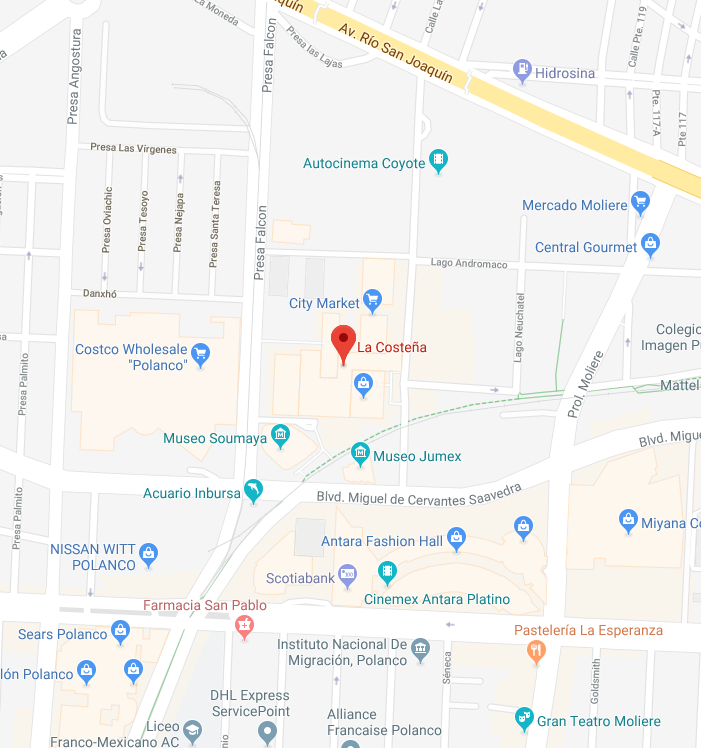
\includegraphics[width=.7\textwidth]{imagenes/corporativo.png}
    \caption{Corporativo.}
\end{figure}

\newpage
\subsubsection{Centro de datos}
Av. 12 No 96 Interior 2, Col. Ignacio Zaragoza, México D.F. CP. 15000.
\\ Coordenadas: 19.41 N, 99.09 W
\begin{figure}[ht]
    \centering
    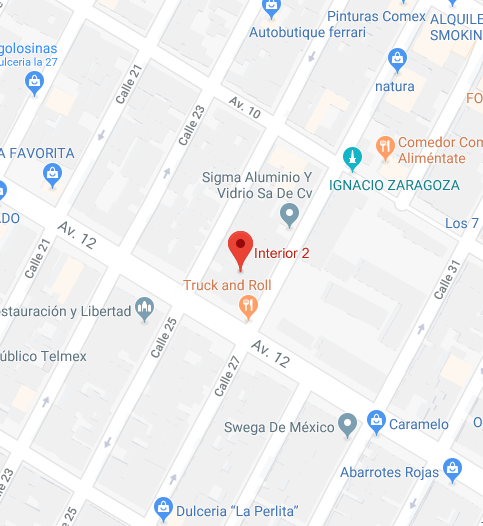
\includegraphics[width=.8\textwidth]{imagenes/centrodatos.png}
    \caption{Centro de datos.}
\end{figure}

\newpage
\subsubsection{Ubicación y niveles por ocupar en el edificio}
\begin{figure}[ht]
    \centering
    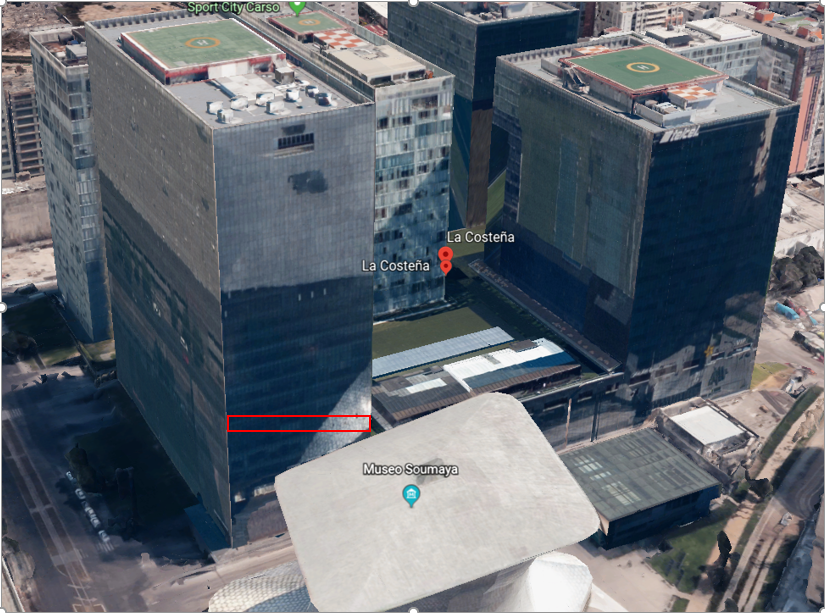
\includegraphics[width=1\textwidth]{imagenes/edificios.png}
    \caption{Plaza Carso.}
\end{figure}
Calle Lago Zurich 245, Amp Granada, 11529 Ciudad de México, CDMX. 
\\ \\
El corporativo esta 
ubicado en plaza Carso, en la torre Frisco/Zurich, piso 7 y 8. Esta 
torre cuenta con una altura de 90m, y 19 pisos de aproximadamente 4.736m de altura.

\newpage
En seguida se muestra la altura en metros de los pisos a ocupar por el corporativo.
\begin{figure}[ht]
    \centering
    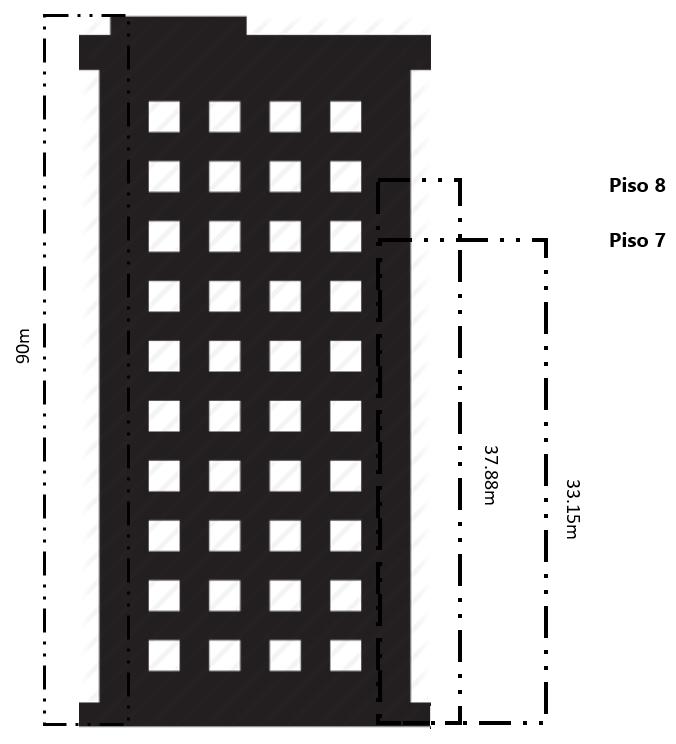
\includegraphics[width=.8\textwidth]{imagenes/torre.png}
    \caption{Plaza Carso.}
\end{figure}

\newpage
\subsubsection{Organigrama}
\begin{figure}[ht]
    \centering
    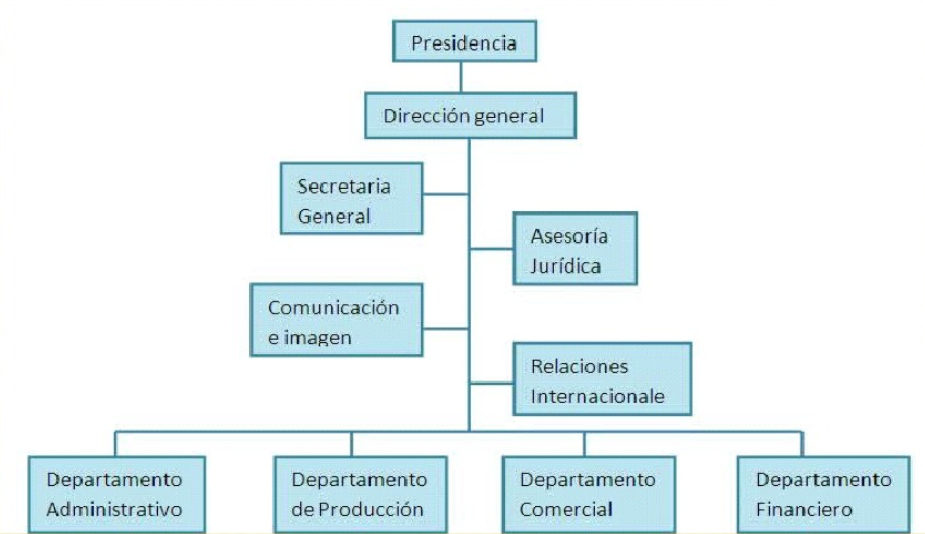
\includegraphics[width=.9\textwidth]{imagenes/organigrama.png}
    \caption{Organigrama. \cite{costenaorganigrama}}
\end{figure}
Personal del corporativo.
\begin{itemize}
    \item \textbf{Presidencia: }
    \item \textbf{Dirección General: }
    \item \textbf{Secretaría General: }
    \item \textbf{Asesoría Jurídica: }
    \item \textbf{Comunicación e Imagen: }
    \item \textbf{Relaciones Internacionales: }
    \item \textbf{Departamento Administrativo: }
    \item \textbf{Departamento de Producción: }
    \item \textbf{Departamento Comercial: }
    \item \textbf{Departamento Financiero: }
\end{itemize}

\newpage
\subsubsection{Detalle arquitectónico}
La Torre de oficinas Lago Zurich está construida en un área de 2130 $m^2$, cuenta con 19 pisos, 
de los cuales 17 se destinan al servicio de oficinas y dos al servicio comercial. Su diseño 
arquitectónico es de tipo moderno. El total de construcción es 36210 $m^2$. \cite{deatllearq} 
El corporativo hace uso de dos pisos en los cuales se distribuyen el total de empleados de la organización con un detalle similar 
al siguiente.
\begin{figure}[ht]
    \centering
    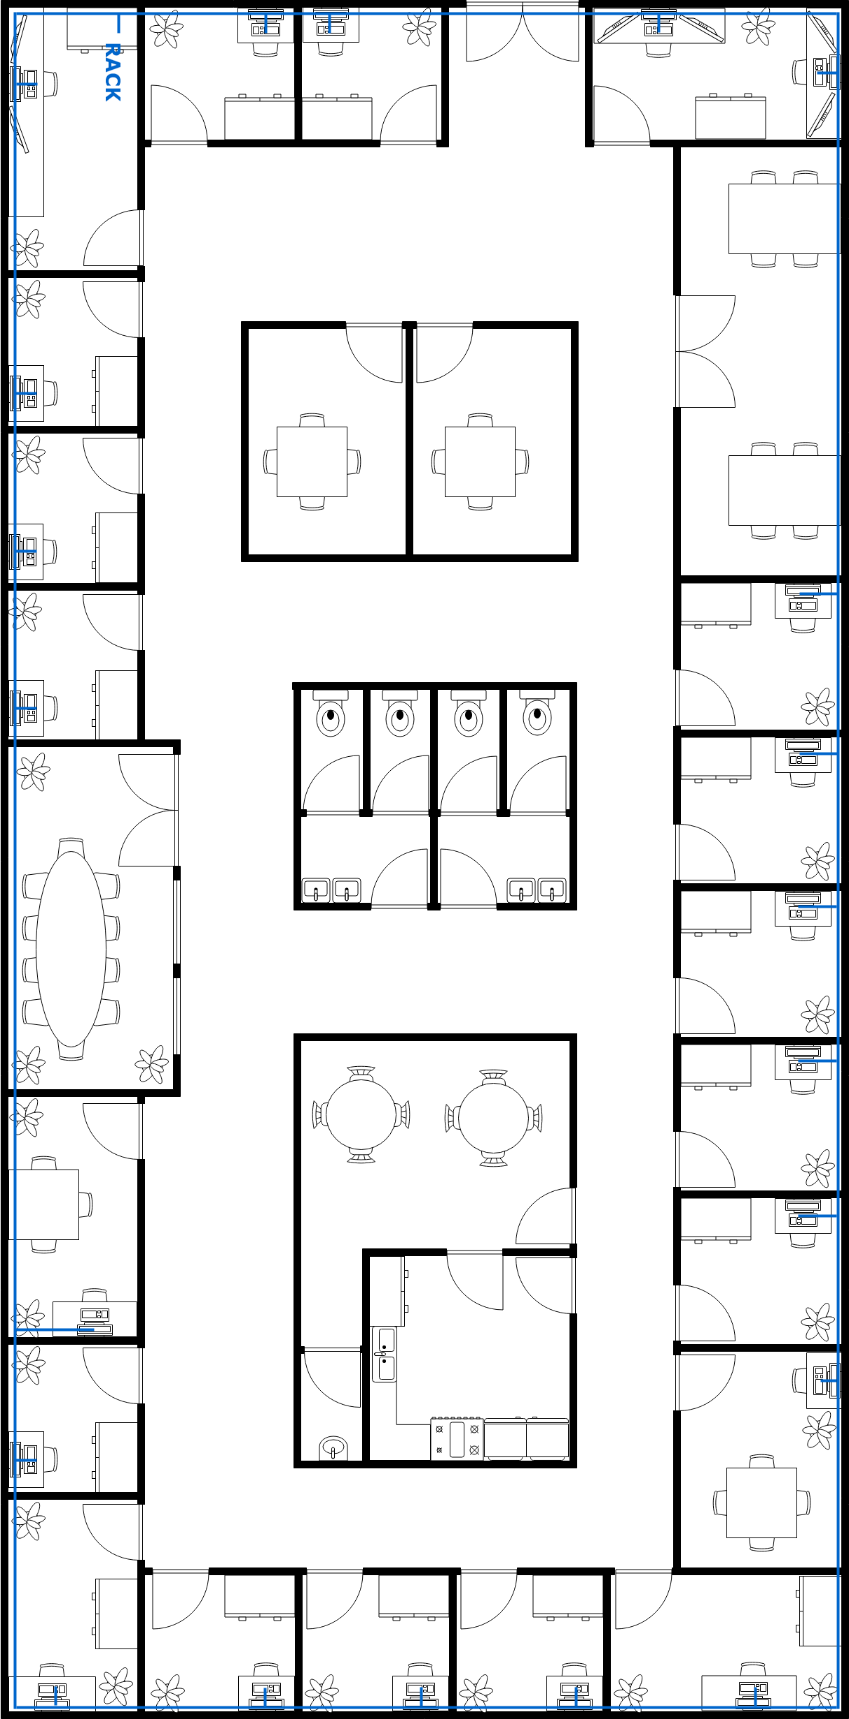
\includegraphics[scale=.75]{imagenes/detalle.png}
    \caption{Detalle de piso.}
\end{figure}

\newpage
\subsection{Ruta Corporativo - Centro de datos }
\subsubsection{Ruta principal y alternativa}
Ruta principal tomando la mayor parte del trayecto por metro.
\begin{figure}[ht]
    \centering
    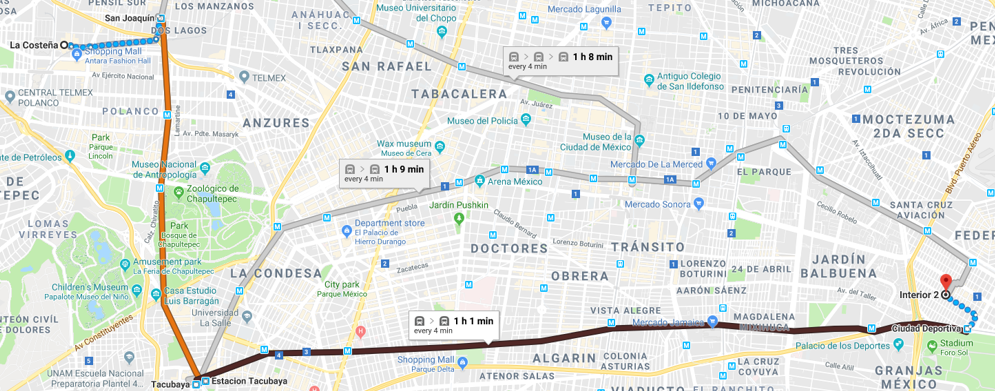
\includegraphics[width=.9\textwidth]{imagenes/f2.png}
    \caption{Ruta principala a escala.}
\end{figure}

La ruta alternativa cuenta con tramo principal por avenidas 
vehiculares.
\begin{figure}[ht]
    \centering
    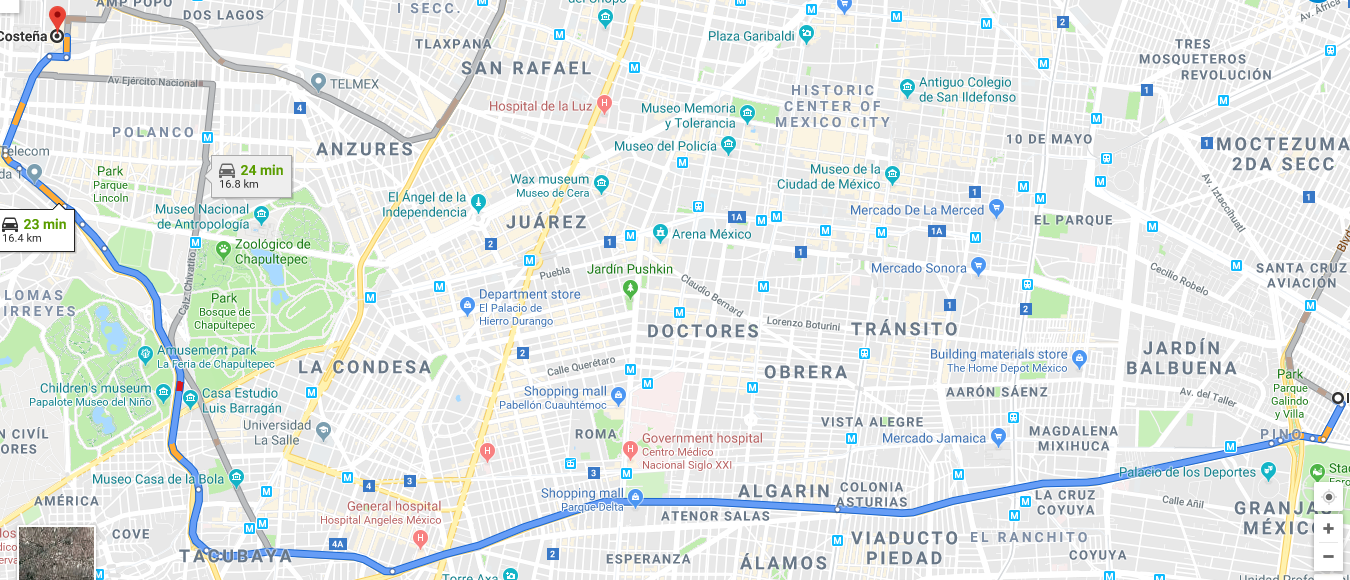
\includegraphics[width=.9\textwidth]{imagenes/f3.png}
    \caption{Ruta alternativa a escala.}
\end{figure}

\newpage
\begin{figure}[ht]
    \centering
    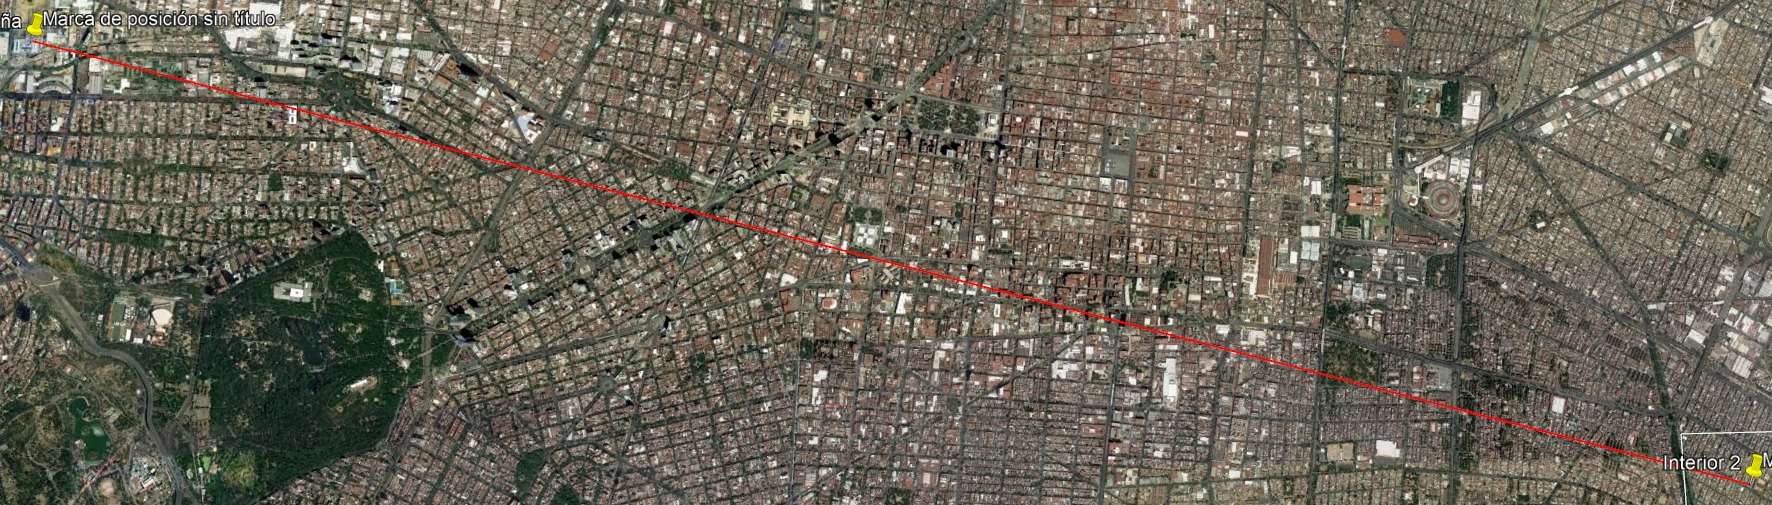
\includegraphics[width=.9\textwidth, angle=90]{imagenes/puntopunto.png}
    \caption{Enlace punto a punto.}
\end{figure}
La distancias son las subsiguientes.
\begin{itemize}
    \item \textbf{Ruta principal: } 16.5 kilometros.
    \item \textbf{Ruta alternativa: } 16.4 kilometros.
    \item \textbf{Punto a punto: } 12 kilometros.
\end{itemize}

\newpage
\subsection{Ruta ISP - Centro de datos}
\subsubsection{Ruta principal y alternativa}
Ruta principal.
\begin{figure}[ht]
    \centering
    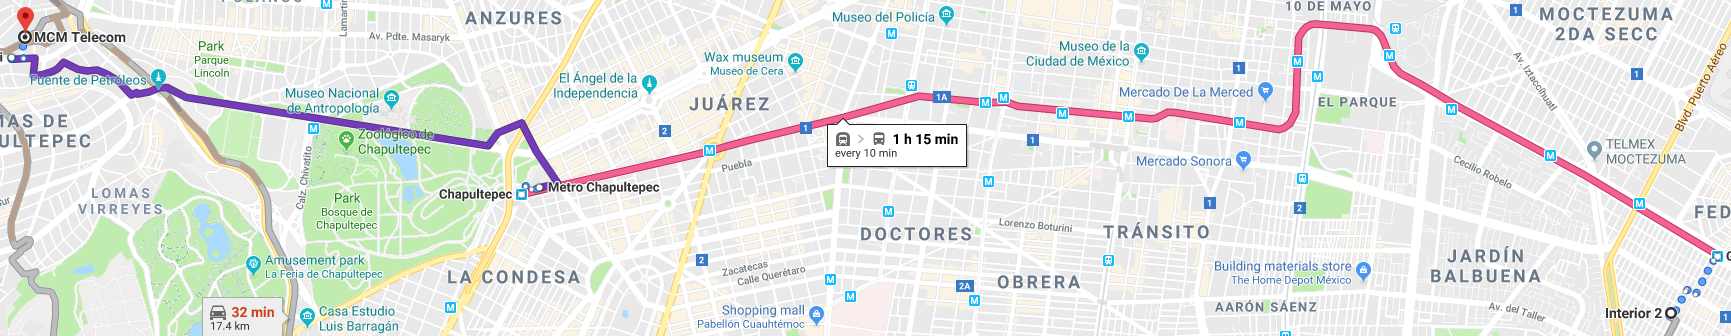
\includegraphics[width=1\textwidth]{imagenes/f22.png}
    \caption{Ruta principal ISP - Centro de datos.}
\end{figure}
\\
Ruta alternativa.
\begin{figure}[ht]
    \centering
    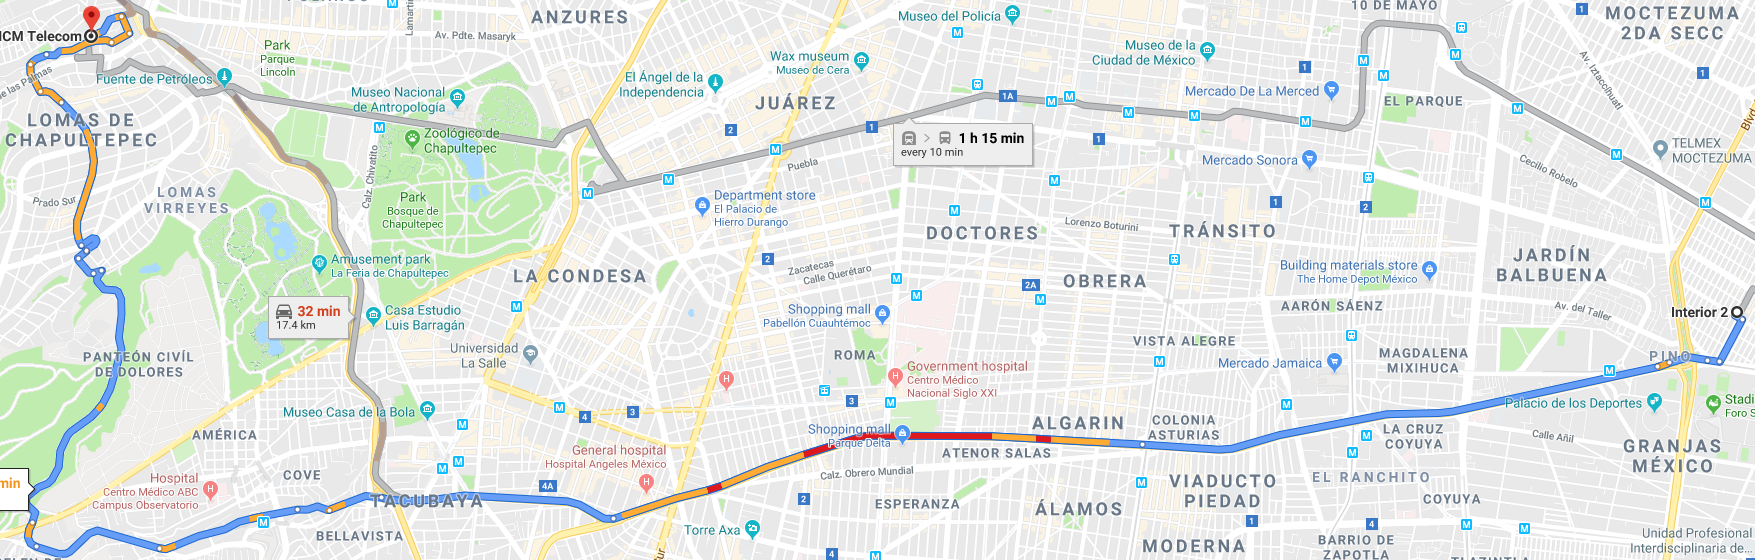
\includegraphics[width=1\textwidth]{imagenes/f23.png}
    \caption{Ruta alternativa ISP - Centro de datos.}
\end{figure}

\newpage
\begin{figure}[ht]
    \centering
    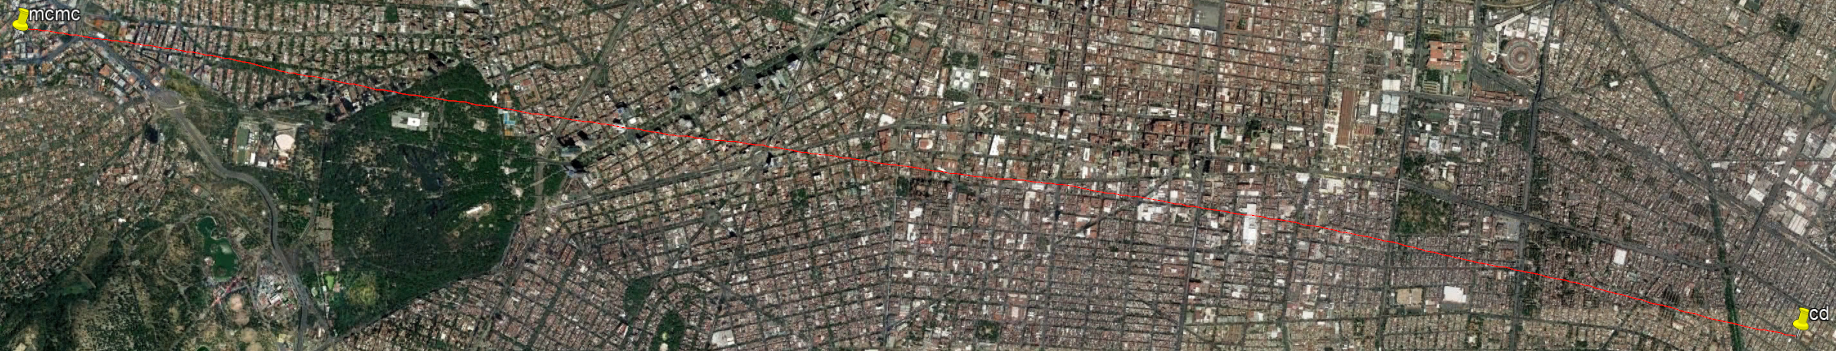
\includegraphics[width=.9\textwidth, angle=90]{imagenes/puntopunto2.png}
    \caption{Enlace punto a punto.}
\end{figure}

La distancias son las subsiguientes.
\begin{itemize}
    \item \textbf{Ruta principal: } 16.5 kilometros.
    \item \textbf{Ruta alternativa: } 16.1 kilometros.
    \item \textbf{Punto a punto: } 12.7 kilometros.
\end{itemize}

\newpage
\subsection{Medios telemáticos}

\subsubsection{Correo electrónico}
El correo electrónico es un servicio de red que permite a los usuarios enviar y recibir 
mensajes (también denominados mensajes electrónicos o cartas digitales) mediante redes de 
comunicación electrónica.
\\ \\
Los sistemas de correo electrónico se basan en un modelo de almacenamiento y reenvío, de 
modo que no es necesario que ambos extremos se encuentren conectados simultáneamente. 
Para ello se emplea un servidor de correo que hace las funciones de intermediario, guardando 
temporalmente los mensajes antes de enviarse a sus destinatarios. \cite{email}

\subsubsection{Video conferencias}
Videoconferencia o videollamada es la comunicación simultánea bidireccional de audio y vídeo, 
que permite mantener reuniones con grupos de personas situadas en lugares alejados entre sí. 
Adicionalmente, pueden ofrecerse facilidades telemáticas o de otro tipo como el intercambio 
de gráficos, imágenes fijas, transmisión de archivos desde el ordenador. \cite{videoConferencia}

\subsubsection{Voice over IP}
Voz sobre protocolo de internet o Voz por protocolo de internet, también llamado voz sobre IP, 
voz IP, vozIP o VoIP, es un conjunto de recursos que hacen posible que la señal de voz viaje 
a través de Internet empleando el protocolo IP. Esto significa que se envía la señal de voz 
en forma digital, en paquetes de datos, en lugar de enviarla en forma analógica a través de 
circuitos utilizables solo por telefonía convencional, como las redes PSTN. \cite{VoIP}
\\ \\ 
El tráfico de voz sobre IP puede circular por cualquier red IP, incluyendo aquellas conectadas 
a Internet, como por ejemplo las LAN.
Es muy importante diferenciar entre voz sobre IP (VoIP) y telefonía sobre IP.
\begin{itemize}
    \item VoIP es el conjunto de normas, dispositivos, protocolos que permite transmitir voz sobre el protocolo IP.
    \item La telefonía sobre IP es el servicio telefónico disponible al público, por tanto, con numeración E.164, realizado con tecnología de VoIP.
\end{itemize}

\subsubsection{Web empresarial}
Un sitio web es un gran espacio documental organizado que la mayoría de las veces está 
típicamente dedicado a algún tema particular o propósito específico. Cualquier sitio web 
puede contener hiperenlaces a cualquier otro sitio web, de manera que la distinción entre 
sitios individuales.
\\ \\ 
No debemos confundir sitio web con página web; esta última es solo un archivo HTML, una 
unidad HTML, que forma parte de algún sitio web. Al ingresar una dirección web, siempre 
se está haciendo referencia a un sitio web, el que tiene una página HTML inicial, que es 
generalmente la primera que se visualiza. \cite{web}

\subsubsection{FTP}
El FTP es un protocolo de red: un conjunto de reglas que establecen cómo deben comunicarse 
dos o más entidades para lograr la transmisión de información. En el caso específico del 
FTP, es un protocolo centrado en la transferencia de archivos a través de una red de tipo 
TCP/IP que se basa en la arquitectura cliente-servidor.
\\ \\ 
El equipo cliente, en este marco, se conecta al servidor mediante el FTP con el objetivo 
de enviar o descargar archivos. Este protocolo busca maximizar la velocidad, sin apelar 
al cifrado para proteger la información. Por eso muchas veces se recurre a aplicaciones 
que posibilitan la transferencia del material, pero con el tráfico cifrado. \cite{ftp}

\subsubsection{Base de datos}
Una base de datos es un conjunto de datos pertenecientes a un mismo contexto y almacenados 
sistemáticamente para su posterior uso. Actualmente, y debido al desarrollo tecnológico de 
campos como la informática y la electrónica, la mayoría de las bases de datos están en 
formato digital, siendo este un componente electrónico, por tanto, se ha desarrollado y 
se ofrece un amplio rango de soluciones al problema del almacenamiento de datos.
\\ \\ 
Existen programas denominados sistemas gestores de bases de datos, abreviado SGBD (del 
inglés Database Management System o DBMS), que permiten almacenar y posteriormente acceder 
a los datos de forma rápida y estructurada. Las propiedades de estos DBMS, así como su 
utilización y administración, se estudian dentro del ámbito de la informática. \cite{basedatos}

\subsection{Protocolos y codec VoIP}
\subsubsection{Protocolo IP}
El protocolo de IP (Internet Protocol) es la base fundamental de la Internet. Porta 
datagramas de la fuente al destino. El nivel de transporte parte el flujo de datos en 
datagramas. Durante su transmisión se puede partir un datagrama en fragmentos que se 
montan de nuevo en el destino. Las principales características de este protocolo son:
\begin{itemize}
    \item Protocolo orientado a no conexión.
    \item Fragmenta paquetes si es necesario.
    \item Direccionamiento mediante direcciones lógicas IP de 32 bits.
    \item Si un paquete no es recibido, este permanecerá en la red durante un tiempo finito.
    \item Realiza el "mejor esfuerzo" para la distribución de paquetes.
    \item Tamaño máximo del paquete de 65635 bytes.
    \item Sólo ser realiza verificación por suma al encabezado del paquete, no a los datos éste que contiene.
\end{itemize}

El Protocolo Internet proporciona un servicio de distribución de paquetes de información 
orientado a no conexión de manera no fiable. La orientación a no conexión significa que los 
paquetes de información, que será emitido a la red, son tratados independientemente, pudiendo 
viajar por diferentes trayectorias para llegar a su destino. El término no fiable significa 
más que nada que no se garantiza la recepción del paquete. \cite{ip}

\subsubsection{Protocolo UDP}
El grupo de protocolos de Internet también maneja un protocolo de transporte sin conexiones, 
el UDP (User Data Protocol, protocolo de datos de usuario). El UDP ofrece a las aplicaciones 
un mecanismo para enviar datagramas IP en bruto encapsulados sin tener que establecer una 
conexión.
\\ \\
Muchas aplicaciones cliente-servidor que tienen una solicitud y una respuesta usan el UDP en 
lugar de tomarse la molestia de establecer y luego liberar una conexión. El UDP se describe 
en el RFC 768. Un segmento UDP consiste en una cabecera de 8 bytes seguida de los datos. La 
cabecera se muestra a continuación. Los dos puertos sirven para lo mismo que en el TCP: para 
identificar los puntos terminales de las máquinas origen y destino. El campo de longitud UDP 
incluye la cabecera de 8 bytes y los datos. La suma de comprobación UDP incluye la misma 
pseudocabecera de formato, la cabecera UDP, y los datos, rellenados con una cantidad par 
de bytes de ser necesario. \cite{udp}

\subsubsection{Protocolo TCP/IP}
TCP/IP es el nombre de un protocolo de conexión de redes. Un protocolo es un conjunto de 
reglas a las que se tiene que atener todas la compañías y productos de software con él fin 
de que todos sus productos sean compatibles entre ellos. Estas reglas aseguran que una 
máquina que ejecuta la versión TCP/IP de Digital Equipment pueda hablar con un PC Compaq 
que ejecuta TCP/IP.
\\ \\
TCP/IP es un protocolo abierto, lo que significa que se publican todos los aspectos concretos 
del protocolo y cualquiera los puede implementar.
\\ \\
TCP/IP está diseñado para ser un componente de una red, principalmente la parte del software. 
Todas las partes del protocolo de la familia TCP/IP tienen unas tareas asignadas como enviar 
correo electrónico, proporcionar un servicio de acceso remoto, transferir ficheros, asignar 
rutas a los mensajes o gestionar caídas de la red.
\\ \\
Una red TCP/IP transfiere datos mediante el ensamblaje de bloque de datos en paquetes. Cada 
paquete comienza con una cabecera que contiene información de control, tal como la dirección 
del destino, seguida de los datos. Cuando se envía un archivo a través de una red TCP/IP, 
su contenido se envía utilizando una serie de paquetes diferentes. \cite{tcp}

\subsubsection{RTCP}
RTP es la abreviación de Real-time Transport Protocol, por su denominación en inglés. Es un 
estándar creado por la IETF para la transmisión confiable de voz y video a través de Internet. 
La primera versión fue publicada en 1996 en el documento RFC 1889 y fue reemplazado por el 
estándar RFC 3550 en 2003.
\\ \\
En aplicaciones de Voz sobre IP, RTP es el protocolo responsable de la transmisión de los 
datos. La digitalización y compresión de la voz y el video es realizada por el CODEC. Para 
el manejo de señalización o establecimiento de llamada existe el protocolo SIP.
\\ \\
Dentro del estándar RFC 3550 se define un protocolo adicional para el envío de datos de 
control y datos de mediciones realizadas durante la transmisión. Se conoce como RTCP RTP 
Control Protocol. los paquetes RTCP se envían periódicamente dentro de la secuencia de 
paquetes RTP. \cite{rtcp}

\subsubsection{PPP}
PPP se utiliza comúnmente como protocolo de capa de enlace de datos para la conexión a través 
de circuitos síncronos y asíncronos, donde ha reemplazado en gran medida a los antiguos 
protocolos de Internet de línea serie (SLIP) y a los estándares exigidos por las compañías 
telefónicas (como el protocolo de acceso de enlace, balanceado (LAPB) en el conjunto de 
protocolos X.25). El único requisito para el PPP es que el circuito suministrado sea dúplex. 
PPP fue diseñado para trabajar con numerosos protocolos de capa de red, incluyendo el 
Protocolo de Internet (IP), TRILL, Internetwork Packet Exchange (IPX) de Novell, NBF, 
DECnet y AppleTalk. Al igual que SLIP, se trata de una conexión completa a Internet a 
través de líneas telefónicas por módem. 
\\ \\
El RFC 2516 describe el Protocolo Punto a Punto sobre Ethernet (PPPoE) como un método para 
transmitir PPP sobre Ethernet que a veces se utiliza con DSL. El RFC 2364 describe el 
Protocolo Punto a Punto sobre ATM (PPPoA) como un método para transmitir PPP sobre ATM 
Adaptation Layer 5 (AAL5), que es también una alternativa común a PPPoE utilizado con DSL.\cite{ppp}
\\ \\
PPP es un protocolo estratificado que tiene tres componentes:
\begin{itemize}
    \item Un componente de encapsulación que se utiliza para transmitir datagramas sobre la capa física especificada.
    \item Un Protocolo de Control de Enlaces (LCP) para establecer, configurar y probar el enlace, así como para negociar la configuración, las opciones y el uso de las funciones.
    \item Uno o más Protocolos de Control de Red (NCP) utilizados para negociar parámetros de configuración opcionales y facilidades para la capa de red. Existe un NCP para cada protocolo de capa superior soportado por PPP.
\end{itemize}

\subsubsection{VAD}
En Voz sobre IP (VOiP), la detección de activación de voz (VAD) es una aplicación de software 
que permite a una red de datos que transporta tráfico de voz a través de Internet detectar la 
ausencia de audio y conservar el ancho de banda evitando la transmisión de "paquetes 
silenciosos" a través de la red. La mayoría de las conversaciones incluyen un 50 prociento 
de silencio; el VAD (también llamado "supresión de silencio") puede habilitarse para 
monitorizar señales de actividad de voz, de modo que cuando se detecta silencio durante un 
tiempo determinado, la aplicación informa al protocolo de voz en paquetes e impide que la 
salida del codificador sea transportada a través de la red.
\\ \\
La detección de activación por voz también se puede utilizar para reenviar las características 
de ruido de ralentí (a veces llamado ruido ambiental o de confort) a un teléfono IP remoto 
o a una pasarela. El estándar universal para voz digitalizada, 64 Kbps, es una velocidad de 
bits constante, ya sea que el hablante esté hablando activamente, esté haciendo una pausa 
entre pensamientos o esté totalmente en silencio. Sin el ruido de ralentí que da la ilusión 
de un flujo de transmisión constante durante la supresión del silencio, es probable que el 
oyente piense que la línea se ha cortado. \cite{vad}

\subsubsection{MPLS}
Conmutación de etiquetas multiprotocolo (MPLS)
La conmutación de etiquetas multiprotocolo (MPLS) es una técnica de enrutamiento agnóstico 
al protocolo diseñada para acelerar y dar forma a los flujos de tráfico a través de las 
redes de área amplia de la empresa y de los proveedores de servicios.
\\ \\
MPLS permite que la mayoría de los paquetes de datos se reenvíen a Nivel 2 - el nivel 
de conmutación - en lugar de tener que pasar al Nivel 3 - el nivel de enrutamiento. Por 
esta razón, a menudo se describe informalmente como operando en la capa 2.5.
\\ \\
MPLS fue creado a finales de los años 90 como una alternativa más eficiente al 
enrutamiento IP tradicional, que requiere que cada enrutador determine independientemente 
el siguiente salto de un paquete inspeccionando la dirección IP de destino del paquete 
antes de consultar su propia tabla de enrutamiento. Este proceso consume tiempo y 
recursos de hardware, lo que puede resultar en un rendimiento degradado para aplicaciones 
en tiempo real, como voz y vídeo.
\\ \\
En una red MPLS, el primer enrutador en recibir un paquete determina la ruta completa 
del paquete por adelantado, cuya identidad se transmite rápidamente a los enrutadores 
subsiguientes utilizando una etiqueta en la cabecera del paquete.
\\ \\
Mientras que el hardware del router ha mejorado exponencialmente desde que se desarrolló 
MPLS, disminuyendo un poco su importancia como una tecnología de gestión de tráfico más 
eficiente, sigue siendo importante y popular debido a sus otros beneficios, en particular 
la seguridad, la flexibilidad y la ingeniería de tráfico. 
\\ \\
\textbf{Componentes de MPLS}
\newline
Una de las características que definen a MPLS es el uso de etiquetas, la L en MPLS. 
Entre las capas 2 y 3, una etiqueta es un identificador de cuatro bytes - 32 bits - 
que transmite la ruta de reenvío predeterminada del paquete en una red MPLS. Las 
etiquetas también pueden contener información relacionada con la calidad de 
servicio (QoS), indicando el nivel de prioridad de un paquete.
\\ \\
Las etiquetas MPLS constan de cuatro partes:
\begin{itemize}
    \item Valor de la etiqueta: 20 bits.
    \item Experimental: 3 bits.
    \item En la parte inferior de la pila: 1 bit.
    \item Tiempo de vida: 8 bits.
\end{itemize}

Los trayectos, que se denominan trayectos con conmutación de etiquetas (LSP), 
permiten a los proveedores de servicios decidir de antemano la mejor manera de 
que determinados tipos de tráfico fluyan dentro de una red privada o pública. \cite{mpls}

\newpage
\subsection{Conectividad enlace ATM}
\begin{figure}[ht]
    \centering
    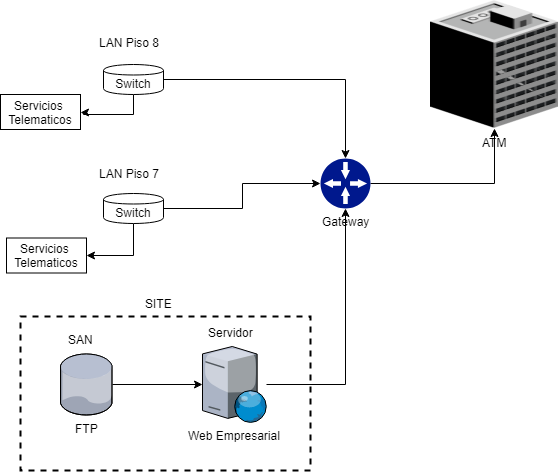
\includegraphics[width=.9\textwidth]{imagenes/atmdia.png}
    \caption{Enlace ATM.}
\end{figure}

\newpage
\subsection{Arquitectura de red (Intra-ATM)}
\begin{figure}[ht]
    \centering
    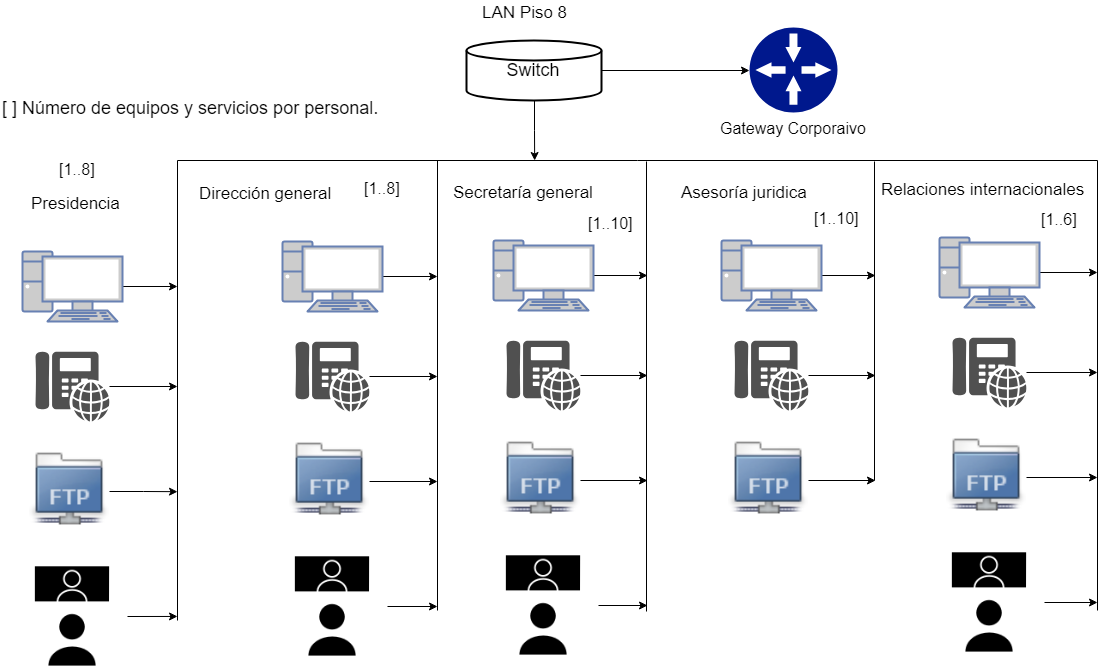
\includegraphics[width=.9\textwidth,angle=90]{imagenes/Lan8.png}
    \caption{Diseño propuesto de la red LAN para el piso 8.}
\end{figure}

\newpage
\begin{figure}[ht]
    \centering
    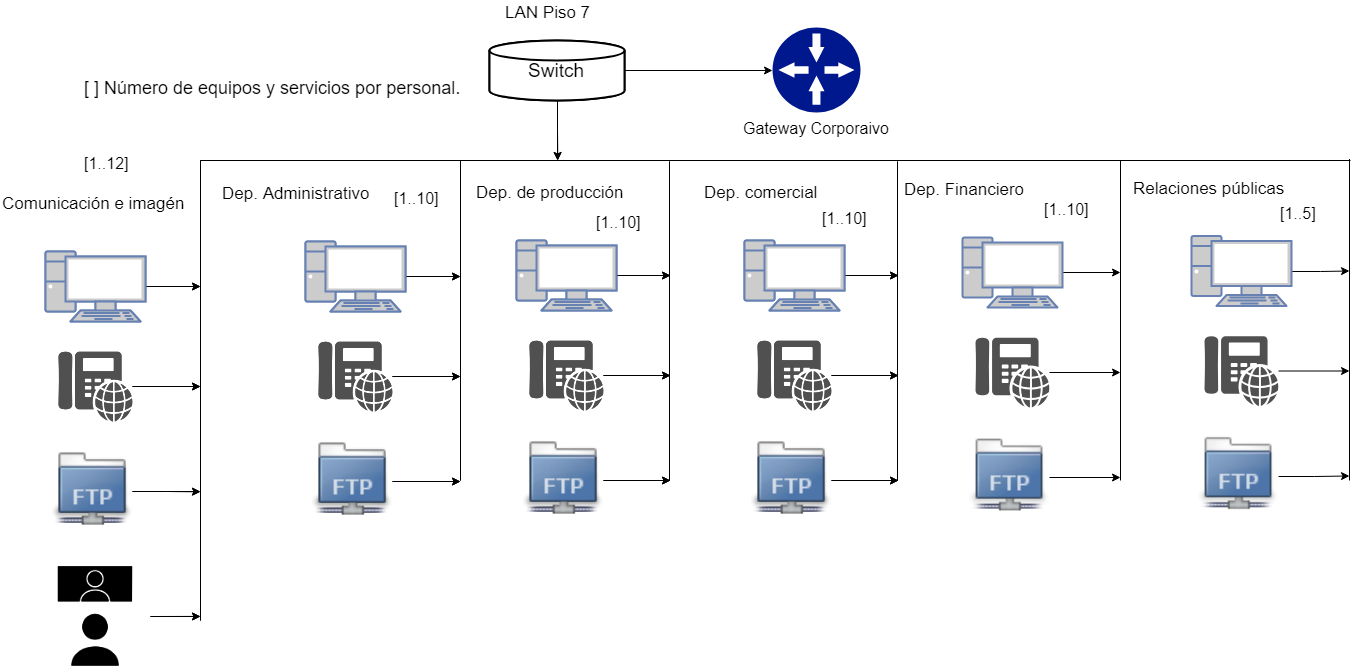
\includegraphics[width=.9\textwidth,angle=90]{imagenes/Lan7.png}
    \caption{Diseño propuesto de la red LAN para el piso 7.}
\end{figure}



\newpage
\section{Planeación}

\newpage
\section{Requerimientos Ecomerce}

\newpage
\section{Cálculo de enlace}


\newpage
\section{Anexos}
\subsection{Cálculos}

\newpage
\begin{thebibliography}{20}
    \bibitem{lacostena} 
    lacostena.com.mx, "Sobre nosotros". 
    [Online] Disponible lacostena.com.mx/es/sobre-nosotros.
    [Ultimo Acceso: 22/02/2019]

    \bibitem{costenaorganigrama}
    $es.scribd.com/presentation/314767015/Empresa-La-Costena$

    \bibitem{deatllearq}
    $edemx.com/citymex/rascacielos/Carso_zurich.html$

    \bibitem{email}
    $whatis.techtarget.com/definition/e-mail-electronic-mail-or-email$
     
    \bibitem{videoConferencia}
    $searchunifiedcommunications.techtarget.com/definition/video-conference$

    \bibitem{VoIP}
    $searchdatacenter.techtarget.com/es/definicion/Voz-sobre-IP-VoIP$

    \bibitem{web}
    $definicion.de/sitio-web/$

    \bibitem{ftp}
    $tools.ietf.org/html/rfc959$

    \bibitem{basedatos}
    $searchsqlserver.techtarget.com/definition/database$

    \bibitem{ip}
    $techopedia.com/definition/5366/internet-protocol-ip$

    \bibitem{udp}
    $searchnetworking.techtarget.com/definition/UDP-User-Datagram-Protocol$

    \bibitem{tcp}
    $techopedia.com/definition/5773/transmission-control-protocol-tcp$

    \bibitem{rtcp}
    $techopedia.com/definition/25807/rtp-control-protocol-rtcp$

    \bibitem{ppp}
    $cisco.com/c/es_mx/tech/wan/point-to-point-protocol-ppp/$

    \bibitem{vad}
    $searchunifiedcommunications.techtarget.com/definition/voice-activation-detection$

    \bibitem{mpls}
    $www.networkworld.es/telecomunicaciones/como-funciona-mpls$

    \bibitem{servidorhp}
    $hpe.com/mx/es/product-catalog/servers/proliant-servers/pip.hpe-proliant-dl580-gen10-server.1010192779.html$

    \bibitem{pdh}
    $es.wikipedia.org/wiki/Jerarquiadigitalplesiocrona$

    \bibitem{ethernet}
    $electronics-notes.com/articles/connectivity/ethernet-ieee-802-3/$

    \bibitem{swicthes}
    $meraki.cisco.com/products/switches/ms120-48$

    \bibitem{routers}
    $meraki.cisco.com/products/wireless/mr42$

    \bibitem{routers2}
    $meraki.cisco.com/products/wireless/mr53$

    \bibitem{gateways}
    $cisco.com/c/en/us/products/collateral/unified-communications/vg-series-gateways/datasheetc78-710996.html$

\end{thebibliography}

\end{document}